%\documentclass[11pt,twocolumn]{article}
%\documentclass[11pt,letter]{article}
\documentclass[11pt]{article}
%\documentclass[10pt]{aastex}

%\documentclass[preprint]{aastex}
\usepackage{graphicx,epsfig,natbib,multicol}
\usepackage{hyperref}
%\usepackage{natbib,epsfig}
%\usepackage{/Users/grudnick/LaTeX/sttools/stfloats}
%\usepackage{fullpage}
%\usepackage{multicol}
\usepackage{wrapfig}
\usepackage{times}
\usepackage{subfigure}
%\usepackage[top=0.5in, bottom=1.5in, left=1.1in, right=0.8in]{geometry}
%% \addtolength{\oddsidemargin}{-.875in}
%% 	\addtolength{\evensidemargin}{-.875in}
%% 	\addtolength{\textwidth}{1.75in}

%% 	\addtolength{\topmargin}{-.875in}
%% 	\addtolength{\textheight}{1.75in}

\usepackage{simplemargins}
\setleftmargin{1.0in}
	\setrightmargin{1.0in}
	\settopmargin{1in}
	\setbottommargin{1.0in}
%	\setallmargins{dimen}
%\setallmargins{1.2in}

%\usepackage[top=0.5in, bottom=1.6in, left=1.1in, right=0.8in]{geometry}
%\usepackage[top=0.7in, bottom=1.2in, left=1.1in, right=1.1in]{geometry}
%\usepackage{onecolfloat}
%\usepackage{epsf}
%\includeonly{references}
\usepackage{macros_rudnick}
\newcommand{\HRule}{\rule{\linewidth}{0.3mm}}
\setlength{\parskip}{3pt}
\setlength{\parsep}{0pt}
\setlength{\headsep}{0pt}
\setlength{\topskip}{0pt}
\setlength{\topmargin}{0pt}
\setlength{\topsep}{0pt}
\setlength{\partopsep}{0pt}

%\addtolength{\parskip}{-4pt}

%\usepackage{pslatex}

\usepackage[compact]{titlesec}
%\titlespacing{\section}{0pt}{*0.2}{*0.2}
%\titlespacing{\subsection}{0pt}{*0.1}{*0.1}
%\titlespacing{\subsubsection}{0pt}{*0.1}{*0.1}

%% %to get EPSCoR page numbering 
%% \usepackage{fancyhdr}
%% \pagestyle{fancy}
%% \fancyhead{}
%% \fancyfoot{}
%% \cfoot[]{C-\thepage}
%% \renewcommand{\headrulewidth}{0pt}

%% % Alter some LaTeX defaults for better treatment of figures:
%%     % See p.105 of "TeX Unbound" for suggested values.
%%     % See pp. 199-200 of Lamport's "LaTeX" book for details.
%%     %   General parameters, for ALL pages:
%%     \renewcommand{\topfraction}{1.0}	% max fraction of floats at top
%%     \renewcommand{\bottomfraction}{1.0}	% max fraction of floats at bottom
%%     %   Parameters for TEXT pages (not float pages):
%%     \setcounter{topnumber}{2}
%%     \setcounter{bottomnumber}{2}
%%     \setcounter{totalnumber}{4}     % 2 may work better
%%     \setcounter{dbltopnumber}{2}    % for 2-column pages
%%     \renewcommand{\dbltopfraction}{0.9}	% fit big float above 2-col. text
%%     \renewcommand{\textfraction}{0.07}	% allow minimal text w. figs
%%     %   Parameters for FLOAT pages (not text pages):
%%     \renewcommand{\floatpagefraction}{0.7}	% require fuller float pages
%% 	% N.B.: floatpagefraction MUST be less than topfraction !!
%%     \renewcommand{\dblfloatpagefraction}{0.7}	% require fuller float pages

%% 	% remember to use [htp] or [htpb] for placement

% Figures within a column...
\makeatletter
\newenvironment{tablehere}
{\def\@captype{table}}
{}
\newenvironment{figurehere}
{\def\@captype{figure}}
{}
\makeatother

\bibpunct[;]{(}{)}{;}{a}{}{,}


\begin{document}
%\maketitle
%\noindent\HRule

%\renewcommand{\thepage}{D--\arabic{page}}

%\everypar{\looseness=-1}


%\hline
%\begin{center}
%Project description
%\end{center}
%\hline

%\begin{multicols}{2}

%\HRule
%\vspace{-1.5in}
\begin{center}
\large{Proposal for an ISSI International Team}\\
\Large{COSWEB: The Cosmic Web and Galaxy Evolution}\\
\medskip
\vspace{-0.2cm}
\large{Coordinator: Gregory Rudnick}\\
\end{center}
%\HRule
We have assembled the COSWEB team to study the interplay between the cosmic web and galaxy evolution. COSWEB is an outgrowth of a previous ISSI project that focused specifically on how the gas content of galaxies is affected by galaxy clusters. We propose to continue our studies of the gas content of clusters as well as exploit a breakthrough our team has made in characterizing the filamentary structure around clusters.

Starting over thirty years ago, astronomers began to suspect that a galaxy's environment affects its evolution.  Compared to the average galaxy, those residing in high density areas have systematically older stellar populations, lower star formation rates (SFR), and  different morphologies.  In the past decade, large surveys of galaxies with ground-based telescopes have cemented the existence of these environmentally-dependent differences. However, the physical mechanisms by which galaxies are altered as they enter dense environments have not yet been conclusively identified and we do not know where different processes dominate.

Two elements are largely missing from current analyses: 1) information about the gaseous fuel for SF and 2) a proper treatment of dense filamentary environments, rather than a simplistic focus on clusters, groups, and field populations. Our team will address these shortcomings by both characterizing the stellar and gaseous contents of galaxies over a large range in lookback time and by focusing much of our effort on studying galaxies in filaments, the site where many galaxies first encounter a dense environment.

%If the relevant physical mechanisms are operating on the gas content of galaxies, and thereby affecting subsequent SF and the resulting effects on morphology, then we must have direct measures of the gas content, physical state, and spatial distribution. Likewise, if (one of) the relevant physical mechanisms operates along filaments that feed into groups and clusters, we may fail to identify it by focusing solely on environmental metrics such as cluster-centric distance or local density. 

We have assembled a team that can address both of these concerns and bring fresh insights to understanding the environmental dependence of galaxy properties. Our team is composed of 12 individuals from six countries whose research expertise as follows (five new members indicated with a '$^*$'):
\vspace{-0.1in}
\begin{itemize} 
%\vspace{-0.1in}
\item \textit{Molecular tracers of star-forming gas:} F. Combes (F), P. Jablonka (CH), G. Rudnick (USA),
A. Noble$^*$ (USA), E. van Kampen$^*$ (DE), M. Cooper (USA)
\vspace{-0.1in}
\item \textit{Ionized tracers of star-forming gas:} B. Weiner (USA), G. Rudnick (USA) R. Finn (USA), Y. Jaffe$^*$ (Chile) 
\vspace{-0.1in}
\item \textit{Dust-obscured star formation:} R. Finn (USA), , G. Rudnick (USA), P. Jablonka (CH)
\vspace{-0.1in}
\item \textit{Galaxy environment:} D. Zaritsky (USA), G. Castignani$^*$ (F), P. Jablonka (CH), M. Cooper (USA), D. Norman$^*$ (USA), Y. Jaffe$^*$ (Chile)
\vspace{-0.1in}
\item \textit{Very distant clusters:} G. Rudnick (USA), B. Weiner (USA), A. Noble$^*$ (USA), E. van Kampen$^*$ (DE), G. Castignani$^*$ (F) 
\vspace{-0.1in}
\item \textit{Theoretical modeling:} G. De Lucia (IT), M. Cooper (USA), F. Combes (F), van Kampen$^*$ (DE)
\end{itemize}
%\vspace{-0.15in}
These individuals are using the largest ground-based telescopes, the best space facilities, and the largest and newest radio/mm interferometers on the planet.  Together they account for much of the data on gas in dense environments, and over a large baseline in cosmic time.  



The immediate goals of our team are to:
\vspace{-0.1in}
\begin{itemize}
\item Use HST  spectroscopic  observations at  intermediate redshift and H$\alpha$ narrow-band imaging of the nearby Virgo cluster to determine the response of the ionized gas to the environmental effects.
% environments by combining results of HST spectroscopic observations of intermediate redshift clusters with H$\alpha$ narrow-banding imaging of Virgo cluster.
%Trace the evolution of the content and spatial distribution of the ionized gas in galaxies in dense environments using HST  spectroscopic  observations at  intermediate redshift and H$\alpha$ narrow-band imaging of the nearby Virgo cluster.
\vspace{-0.1in}
\item Determine how the SFR and dust content are
  affected by environment through the use of \spitzer, WISE, and \herschel\ observations of
  dust emission in addition to interferometric observations of
  the molecular gas content in filaments and galaxy clusters spanning 10~Gyr of
  cosmic time.
\vspace{-0.1in}
\item Compare the spatial distribution of the different gas phases to that of the stars to constrain the environmental mechanisms that suppress star formation and change galaxy morphology.
\vspace{-0.1in}
\item Initiate new observational programs using JWST and millimeter interferometers to measure the detailed spatial distribution of the ionized and molecular gas of distant filament and cluster galaxies and compare how each phase responds to galaxy environment.
\vspace{-0.1in}
\item Constrain models of environmental gas depletion in simulated galaxies that are evolving in a universe characterized by hierarchical structure growth.
\end{itemize}
\vspace{-0.1in}

%This team includes experts who are working on the identification of filaments in both the nearby universe and at intermediate redshifts; on the properties of the dust content of galaxies using the Spitzer Space Telescope; on the distribution of SF and ionized gas using the Hubble Space Telescope and the largest optical ground-based telescopes (GTC); and on the distribution of the cold gas using the largest and newest radio interferometers on the planet (JVLA, PdBI, ALMA).  The group also includes theorists to simulate the observational effects of different environmental mechanisms, enabling a quantitative interpretation of the data. The purpose of this proposal is to bring this team together to synthesize results and bring unique data and expertise to bear on the problem of how dense environments, particularly filaments, affect the gas components of galaxies, and what physical processes are responsible for it.

\newpage

\centerline{{\bf \underline{ The Role of Environment in Galaxy Evolution: our past and future activities}}}
\medskip

This is an extension proposal for our previous ISSI team ``The Effect of Dense Environments on Gas in Galaxies over 10 Billion Years of Cosmic Time" (PI Rudnick) which produced eight papers, 10 accepted telescope proposals, and one accepted NASA funding proposal.   In addition to our significant success in gathering new data and funding resources we also started a new research area that grew out of the initial ISSI work.  Exploiting these new data, bringing the new research area to fruition, and synthesizing all the results requires support from ISSI in the form of a renewal proposal.  Our new team requires the expertise of five new members. 

\indent{\bf A new focus on how the gas within galaxies is altered within Filaments:} Galaxies in dense environments
have lower average SF rates than field galaxies out
to at least $z \sim 1$ \citep[e.g.][]{Poggianti99,Lewis02,Gomez03,Postman05}.
However, it
is still not clear whether the clusters actively alter the gas content
of infalling galaxies or whether they are the final resting place of
dead galaxies whose gas was depleted before entering the cluster
environment.

At low and intermediate redshifts, the suppression of SF starts at large distances from cluster cores, within groups and filaments \citep{Lewis02,Gomez03,Laigle17}.  This is consistent with simulations that show a boosting of ram pressure within filaments \citep{Bahe13}, through which the bulk of the mass flows into the cluster \citep{Ramachandra15}. In contrast, spiral galaxies
in the Virgo cluster core show evidence of cold gas stripping and truncated
gas disks
\citep{Koopmann98,Koopmann04,Dale01,Crowl05,Chung07}.  This
demonstrates that the cluster environment is actively altering the
star-formation properties of at least some of the infalling galaxies.  

To conclusively determine the cause for the
end of SF in dense environments and where it occurs it is important to \textbf{1)} study
the fuel of SF itself and {\bf 2)} probe a large sample of galaxies in the filaments surrounding clusters, as these galaxies are experiencing environmental effects for the first time.  The first goal was the focus of our last ISSI proposal, which we now propose to extend both to synthesize our results and to begin projects with new facilities. The second goal has been largely accomplished by our team, but needs to be folded into our analysis of the gas properties of galaxies.

\indent{\bf A revolution in our characterization of filaments:}  Galaxy environment studies in the past 25 years have focused on a simple trilogy of field, group, and cluster environments.  We have moved beyond these categories by characterizing galaxies within filaments out to lookback times of 6 billion years.

The region around the Virgo cluster is ideal because at $\sim 16$~Mpc,  it is near enough to allow spatially resolved studies, and to benefit from existing shallow, wide surveys. Taking advantage of the massive investment of SDSS spectroscopy over $\sim 5000$deg$^2$, \citet{Kim16} have identified seven well-defined filaments around the Virgo cluster (Fig. 1, left panel), which we now target.

We have also made breakthroughs in our understanding of the filaments feeding distant galaxy clusters at $z>0.4$ thanks to our concerted Spatially Extended ESO Distant Cluster Survey (SEEDisCS) program.  These advances have come thanks to the availability of 1~deg$^{2}$ field of view imagers on 4-meter telescopes that have enabled distant filaments to be identified via accurate photometric redshifts and subsequently be confirmed with multi-object spectroscopy on 6--8-meter class telescopes \citep[Fig. 1, right panel;][]{Rerat17}.  It has taken years to amass this data but we now have the first ability to study highly pure samples of filament galaxies many virial radii away from clusters, in the regions where they may experience environmental affects for the first time.

\begin{figure}[t!]
\vspace{-1cm}
\begin{minipage}{.5\textwidth}
  \centering
  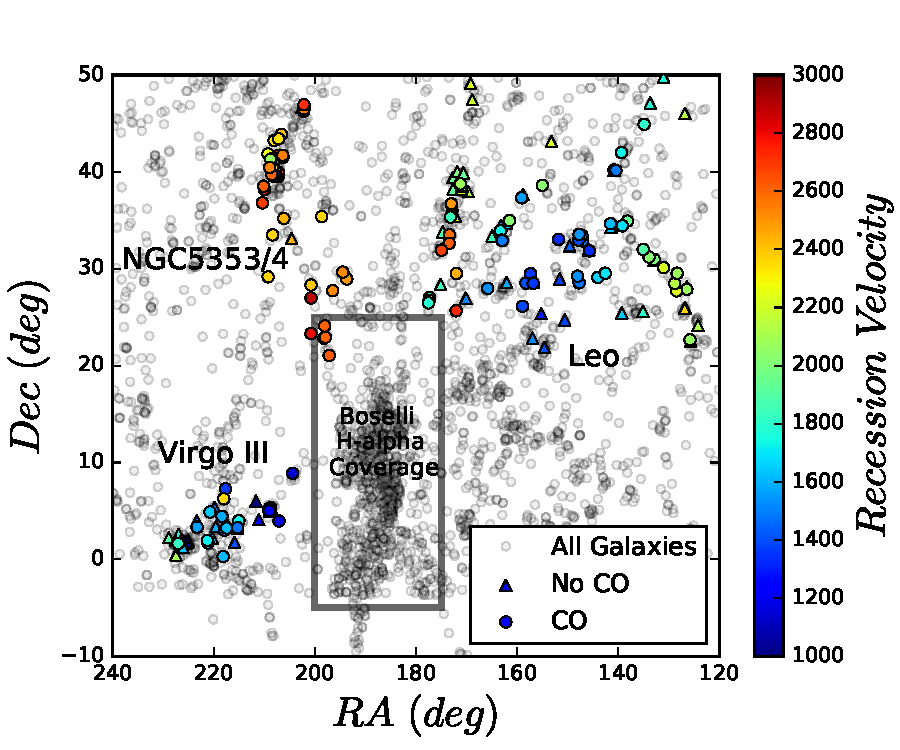
\includegraphics[width=1.0\linewidth]{filaments-for-issi-prop.pdf}
\end{minipage}%
\begin{minipage}{.5\textwidth}
  \centering
  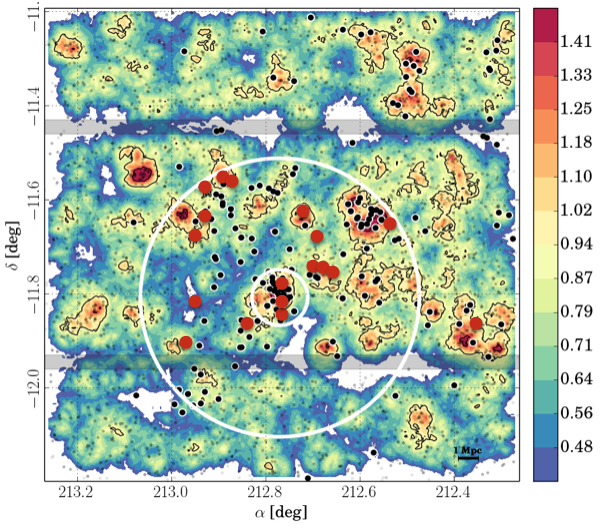
\includegraphics[width=.9\linewidth]{seediscs_filament_with_alma.png}
\end{minipage}
\vspace{-0.5cm}
\caption{\small{{\it Left panel - } Our sample of filaments around the Virgo cluster.  Galaxies we have already observed in CO are shown color-coded by their velocity and split into sources with (circles) and without (triangles) CO detections.  All of these sources have HI observations and will have H$\alpha$ images taken during the timeframe of our ISSI team through already approved programs.  We are also beginning spatially resolved mapping of the CO for a subset of our CO detections.  Other galaxies around the Virgo cluster from \citet{Kim16} are shown in gray.   The Leo filaments are made up of multiple distinct filaments.  Our data will complement the wealth of data available in the Virgo core (gray rectangle). {\it Right panel - } Filamentary structure around a well-studied cluster at z=0.52 drawn from the SEEDisCS sample.  The color-scale shows the density of sources as measured from photometric redshifts.  The black dots are spectroscopically confirmed members and the red dots show sources with ALMA CO observations.  \textit{By combining observations of multiple gas phases our ISSI team will gain a unique view of how filaments affect the gas in galaxies over 5 billion years of cosmic time.}}}
\label{fig:Fig1}
\vspace{0.2cm}
\hrule
\vspace{-0.5cm}
\end{figure}


%\begin{figure}
%\includegraphics[clip=true,trim=0mm 0mm -15mm 0mm,width=6in,angle=0]{virgo_filament_placeholder.png}
%\caption{This is a placeholder caption about the Virgo filaments and SEEDisCS filaments.}
%\end{figure}

%\textbf{The importance of understanding the gas:} Through decades of
%work it has become clear that local supply of cold (mostly molecular)
%gas determines the SFR of galaxies
%\citep{Kennicutt98b,Bigiel08,Leroy08}. Therefore, to truly understand
%how the SFRs of galaxies are altered it is necessary to directly probe
%the content and spatial distribution of the gas.
%
%Different phases of the gas yield complementary information.  The
%content and distribution of ionized gas traces the star formation that
%is relatively unobscured by dust while the mid-infrared emission tells
%us about the obscured star formation.  Likewise, observations of the
%molecular gas constrain the fuel of star formation and its physical
%conditions, i.e. temperature, density, and filling factor.  Although
%the mass of molecular gas is dominated by $H_2$, which has little
%accessible emission due to its lack of a permanent dipole moment and is only visible in shocked gas, we
%can use well-calibrated proxies, such as rotationally excited CO.
%
%It is important to study the amount of gas and its spatial
%distribution with respect to that of the stars.  A key difference
%between the studies of the Virgo core and other local SDSS results mentioned previously is that the
%Virgo studies are based on spatially resolved \ha, CO, or HI maps while
%the others are insensitive to processes that preferentially affect the
%outer radii of galaxies.  This is an important distinction as the most
%common mechanisms proposed for depleting gas make different
%predictions for the size and symmetry of the gas and stars disks.
%
%In addition, studying spatially-resolved gas and stellar disks {\em in filaments as well as in groups and clusters} can help constrain the relative importance
%of physical processes such as ram-pressure stripping, starvation, or tidal effects, because their effectiveness varies with
%the density of the intra-cluster, intra-group medium, or intra-filament gas and the
%velocity of galaxies relative to each other and that gas.  For example, the removal of cold disk gas through
%ram-pressure stripping is expected to be most effective in the cluster
%core, whereas galaxy-galaxy interactions, which exhaust the gas supply
%through a burst of star-formation, are most effective in groups or
%cluster outskirts.  However, galaxies can still experience a 10--100 factor boost in ram pressure stripping in filament environments as they move through the filament gas \citep{Bahe13}.
%
%In a preliminary study, we have found potential signed of gas stripping in that star-forming galaxies in
%clusters appear to have had some of their molecular gas stripped while
%leaving their SFRs - fueled by the densest gas - unaffected for a time
%\citep{Jablonka13}.  While suggestive, these conclusions are based
%primarily on local samples, which have numerous problems.  Locally we can spatially resolve the gas to look for stripping effects.  At intermediate redshift we can also effectively look for environmental effects
%because galaxies are still actively evolving.  Despite this early progress, the number of
%CO measurements in dense environments at intermediate redshift and in filaments at all redshifts is very small and our efforts at
%enlarging them have just started.  

%%\textbf{A revolution in our knowledge of the gas:} To understand how SFRs are altered, we require direct probes of the content and spatial distribution of the gas, which depending on its phase either traces active sites of SF or its fuel supply  \citep[e.g.][]{Kennicutt98b,Bigiel08,Leroy08}. 
%%
%%We are entering a new age of possibility in our ability to study how gas is affected by
%%dense environments thanks to space-based (\spitzer, \herschel, WISE, HST,
%%JWST) and ground-based (ALMA, IRAM, NOEMA, JVLA, VLT, Nancay)
%%observatories.  With slitless spectroscopy
%%observations with HST we are obtaining detailed spatial
%%maps of SF in clusters and their infall regions for
%%systems at $z<0.6$.  HST grism spectroscopy is allowing us to probe
%%the ionized gas and stellar populations of a sample of the most
%%distant clusters at redshifts $z>1.5$.  \spitzer, WISE, and \herschel\ have
%%also given us views of the obscured SF of galaxies back to
%%the early epochs of time.  Locally they allow us to map the relative
%%spatial distribution of the dust and the stars, thus tracing the
%%stripping of the cold gas.  CO observations at the JVLA, IRAM, NOEMA,
%%and ALMA are enabling us to directly measure the content of molecular
%%gas in filament galaxies and we can access HI with JVLA and the Nancay telescope.  Finally, with ALMA and NOEMA we will measure the spatial distribution of molecular gas in
%%galaxies, thus directly probing the physical conditions of star
%%formation as they interact with dense environments.
%%
%%Each of our proposed team members is leading 1--2 of the efforts
%%described above.  We will bring together these resources to
%%address the following questions: In what environment moving from the
%%field, into filaments and groups, and into cluster cores is the gas of galaxies
%%first affected?  How are the content, distribution, density,
%%and temperature of the gas altered?  Over what timescales does the
%%depletion occur?  What are the responsible mechanisms for the gas
%%removal and how do they operate in different environments?  

\centerline{{\bf \underline{ Our proposed activities}}}
%\medskip

\textbf{A revolution in our knowledge of the gas:} To understand how SFRs are altered, we require direct probes of the content and spatial distribution of the gas, which, depending on its phase, either traces active sites of SF or its fuel supply  \citep[e.g.][]{Kennicutt98b,Bigiel08,Leroy08}.  Fortunately, we are in an age of possibility in our ability to study how gas is affected by dense environments, thanks to space-based (\spitzer, \herschel, WISE, HST, JWST) and ground-based (ALMA, IRAM, NOEMA, JVLA, VLT, Nancay) observatories and large observational efforts using these facilities, many of which have been executed by our team members.

We have largely characterized the environments of our galaxies and our immediate work is now to study specific phases of the gas through a set of well-defined programs, described below.  Each of our proposed team members is leading 1--2 of these efforts.  We will bring together these resources to address the following questions: In what environment moving from the field, into filaments and groups, and into cluster cores is the gas of galaxies first affected?  How are the content, distribution, density, and temperature of the gas altered?  Over what timescales does the depletion occur?  What are the responsible mechanisms for the gas removal and how do they operate in different environments?  

%Collectively our team members are studying the both densest environments over 10~Gyr of cosmic time and also the extended cosmic web that feeds those dense environments.  
%A main goal of our proposed ISSI team is to bring all of these results together to form coherent and broad-reaching conclusions with the data that have been provided by the new facilities.


%  The analysis of individual datasets, which usually focus on an individual environment, redshift, or gas phase, will be primarily done by the PIs of those programs.  
%Collectively our team members are studying the both densest environments over 10~Gyr of cosmic time and also the extended cosmic web that feeds those dense environments.  
%A main goal of our proposed ISSI team is to bring all of these results together to form coherent and broad-reaching conclusions with the data that have been provided by the new facilities.

%Studying spatially-resolved gas and stellar disks {\em in filaments as well as in groups and clusters} can help constrain the relative importance of physical processes such as ram-pressure stripping, starvation, or tidal effects, because their effectiveness varies with
%the density of the intra-cluster, intra-group medium, or intra-filament gas and the velocity of galaxies relative to each other and that gas.  For example, the removal of cold disk gas through ram-pressure stripping is expected to be most effective in the cluster
%core, whereas galaxy-galaxy interactions, which exhaust the gas supply through a burst of star-formation, are most effective in groups or cluster outskirts.  However, galaxies can still experience a 10--100 factor boost in ram pressure stripping in filament environments as they move through the filament gas \citep{Bahe13}.  We therefore must probe multiple phases of the gas in a range of environments.

\textit{Ionized gas:} We will determine the effect of environment on the dense ionized
gas by combining an HST/WFC3 grism Cycle 20 program
(PI: Rudnick) on the infall regions of 4 intermediate redshift
clusters with a narrow-band imaging survey of Virgo filament galaxies (PI: Finn).  With these programs
we will distinguish between different methods of gas depletion by
determining relative structure of the star-forming and stellar disks.
For example, ram-pressure stripping makes the prediction that the gas
disks will be asymmetric \citep[e.g.][]{Quilis00,Crowl05} with respect
to the stars and that the SFRs in the inner parts of the galaxy should
be the same as or even enhanced with respect to field galaxies
\citep{Koopmann04,Weinmann10}.  Galaxy-galaxy interactions, however,
will result in both the gas and stars being asymmetric.  Finally,
starvation, which describes a weaker version of ram-pressure stripping
\citep[e.g.][]{Larson80}, may only affect the relative sizes of the
gas and stellar disks.  Our team will propose with JWST grism spectroscopy to obtain spatially resolved maps of Pa$\alpha$ emission ($\lambda=1.875$\micron), which provides an extinction-free measure of the instantaneous SF and which is only available through~JWST.
%By comparing the \ha\ properties of the filament galaxies to those in clusters and infalling groups, we will be able to determine if the filament and group environments are hosting processes that are important in altering star-forming galaxies and how how that role has evolved over
%the last 5~Gyr.

%.  By combining these studies over a large range in redshift and
%cluster or group mass our ISSI team will be able to determine how
%stripping processes have evolved over the last 5~Gyr.

\textit{Obscured star formation:} Infrared observations from
\spitzer, WISE, and \herschel\ probe the emission by dust grains that have
been heated by young stars and can be used to infer the total
infrared luminosity \lir\ and SFR.  
%At
%$z<2$ it is clear that the total SFR in cluster galaxies has declined
%faster than the field \citep{Finn10,Saintonge08,Tran10,Alberts14}.  It is not clear, however, whether this is because evolution in early clusters is ``accelerated" \citep{Papovich12} or because the cluster environment speeds up the
%depletion of gas at late times.  
To isolate the density at which the SFR is first modified in the cosmic web we will use completed wide-field
\spitzer\ 24\micron\ observations around 11 clusters at $0.6<z<0.8$
(PI Rudnick) to measure whether there is a location at which the
fraction of vigorously star-forming galaxies drops.  We will also use our
\spitzer\ 24\micron\ observations of 9 local groups and clusters (PI Finn; Finn et al. 2017) and WISE 12 and 22\micron\ observations of Virgo filament galaxies (PI Finn) to
compare the spatial distribution of the dust emission in galaxies to
that of their stars.  Active stripping of the dust, which is usually co-spatial with the cold gas, will
result in a spatial offset of the dust emission from the stellar
light, while a mere decoupling of the galaxy from its gas supply will
result in a lower mean intensity and smaller  size of the dust emitting region.

\textit{The fuel for star formation.} To truly understand the
modulation of SF by reduction in the H$_2$ fuel supply
requires that we observe the cold gas, or at least a good tracer like CO.  
%Thanks to dramatic technological advances in
%millimetric interferometry with JVLA, NOEMA, and ALMA and the sensitivity if the IRAM 30m telescope we are now able
%to study CO over the full redshift range in which clusters are
%growing.  
%In a preliminary study, we have found that star-forming galaxies in
%clusters appear to have had some of their molecular gas stripped while
%leaving their SFRs - fueled by the densest gas - unaffected for a time
%\citep{Jablonka13}.  While suggestive, however, these results are not conclusive as the local samples have numerous shortcomings.
As part of the efforts initiated by our previous ISSI team we have embarked on an ambitious observational campaign to search for stripping by imaging Virgo filament galaxies in CO, both with the IRAM 30m dish and with the NOEMA interferometer.   We have also made excellent progress on increasing the number of CO detections in intermediate redshift clusters and their surrounding filaments using NOEMA \citep{Jablonka13} and ALMA observations (Jablonka in prep.) and our ISSI team will follow these detections up with spatially resolved observations in future ALMA cycles.  We will also apply for JWST observations to measure H$_2$~directly.  

As the result of JVLA and ALMA programs, team members have now detected CO
in 13 galaxies that reside in four well studied $z\sim 1.6$ proto-clusters
(Rudnick et al. submitted to ApJ; Noble et al. in prep).  Taken together with our intermediate
redshift measurements, these programs comprise most of the CO
detections in dense environments outside the nearby universe.  Part of
our ISSI program will be to combine these studies to measure how
molecular gas and SF relate in dense environments since
$z<2$.  
%CO measurements for field galaxies are rapidly increasing, promising a perfect field comparison sample.
%This is a particularly important part of our project as it gets to the
%heart of what is driving star formation and its cessation, namely the
%molecular gas and its depletion.

\textit{Crucial constraints from observations for theoretical models.} Our
ISSI team includes experts in both semi-analytic models and hydrodynamic simulations.  In nearly all of these
models, the gas supply to galaxies is cut off upon their entry to
another more massive dark matter halo.
%The exact mechanism for this ``satellite quenching'' is unspecified in the models but is parameterized as a timescale for the cutoff of the gas supply.  
Our observations will reveal where the gas supply is cut off, i.e. filaments, the virial radius, cluster core, in groups, and how fast it is shut off.  Current
attempts result in uncomfortably
long quenching timescales, which is how quenching is parameterized in the models \citep{McGee11,DeLucia12a}. The fundamental
problem is that the models don't properly treat the unknown quenching mechanism.
%and have tried to compensate by relaxing the instantaneous cutoff of gas accretion and by including a treatment of non-instantaneous recycling and a partition of the cold gas into atomic and molecular phases \citep{Xie16}.  
Our spatially-resolved study of gas and stellar disks {\em in filaments as well as in groups and clusters} will help constrain the relative importance of physical processes such as ram-pressure stripping, starvation, or tidal effects, because their effectiveness varies with
the density of the intra-cluster medium, intra-group medium, or intra-filament gas and the velocity of galaxies relative to each other and that gas. 
We will thus make crucial steps towards understanding the long debated nature of environmental quenching.

%\textit{Elucidating measurements with revolutionary facilities:}
%ALMA and NOEMA open a new door to
%spatially resolved studies of the cold gas and JWST will allow
%the high spatial resolution of the ionized gas for the first time out to high redshift.  Our ISSI team has been successful proposing for ALMA to and will build on these efforts with the submission of a proposal to make the first significant census of CO in clusters at $z\sim 1.6$.  Thanks to its large wavelength range and 3D spectral capabilities, JWST will allow us to probe the ionized gas in our intermediate and high redshift samples, at wavelengths unencumbered by extinction (Pa$\alpha$, $\lambda=1.875$\micron).  For our nearby galaxies it will also give us the capability to measure H$_2$ directly, and thus measure the bulk of the cold gas without relying on CO as a proxy.  
%A timely effort in the design of these programs is crucial, as JWST has a limited mission lifetime and the first call for proposals is March 2018, right within the timeframe of this proposed team.  
%Likewise, given ALMA's advanced stage of completion, our ISSI team
%is in a perfect position to propose large programs to study the
%cold gas.  A priority of this team will be observing filament galaxies and distant clusters with HST, ALMA, and JWST.

\textbf{Why is our project powerful?}   Collectively, our team has
access to the ideal data to address the questions outlined in our
proposal.  Our filament sample spans $\sim 5~$Gyr of cosmic time while our cluster sample spans $\sim10~$Gyr and
includes the highest redshift cluster with both extremely deep HST
grism data (Lee-Brown et al. 2017), along with one of the largest sample of CO detections in distant clusters (Rudnick et al. 2017; Noble et al. in prep.)  Importantly, our distant clusters are ideally
suited for evolutionary studies as they are all typical progenitors of
our local clusters (Milvang-Jensen et al. 2008; Rudnick et al. 2012).
At intermediate redshift we probe far enough out in clustercentric
radius to identify all of the members that will end up in the cluster
at $z=0$ (Just et al. 2014).  At low redshift we use the proximity of Virgo and other local clusters to probe to low stellar masses where environmental quenching is thought to be dominant and we access HI, CO, Ionized gas, dust, and stellar mass in all of our target galaxies. 

Our proposed collaboration will also probe nearly all of the phases of
the gas that are relevant for SF, from the hot dense gas
that traces active SF to the cold molecular gas that is
the fuel of SF.  We also probe all relevant densities in the cosmic web, from distant filaments to the bottom of deep cluster potential wells.  By combining  measurements with
theoretical models we will gain an improved understanding of
how SF is regulated, and eventually quenched, in dense
environments.  This synergy of the appropriate data and sample, spanning a large range in redshift, and with
accompanying theoretical modeling is unique.


%\textbf{Our proposed team:} Our team is composed of 15 highly
%recognized experts in various areas of galaxy evolution studies and
%represents 7 countries.  They are playing key roles or are leading
%projects in one or more of the areas mentioned
%above. $\bullet$~\textit{Molecular tracers of star-forming gas:}
%F. Combes (F), P. Jablonka (CH), G. Rudnick (USA),
%A. Noble (USA), E. van Kampen (DE), J. Hodge (NL), C. Papovich (USA), M. Cooper (USA) $\bullet$~\textit{Ionized tracers of star-forming gas:}
%B. Weiner (USA), G. Rudnick (USA)
%R. Finn (USA), Y. Jaffe (Chile) $\bullet$~\textit{Dust-obscured star formation:} R. Finn
%(USA), V. Desai (USA), G. Rudnick (USA), C. Papovich
%$\bullet$~\textit{Galaxy environment:} D. Zaritsky (USA), G. Castignani (F), V. Desai (USA), P. Jablonka (CH), M. Cooper (USA), D. Norman (USA), Y. Jaffe (Chile) $\bullet$~\textit{Very distant clusters:} G. Rudnick (USA), B. Weiner
%(USA), A. Noble (USA), E. van Kampen (D), C. Papovich (USA), G. Castignani (F) $\bullet$~\textit{Theoretical modeling:} G. De
%Lucia (IT), M. Cooper (USA), F. Combes (F).  This group has six new members, who bring essential expertise to our collaboration.  This group is larger than 12 but we expect that some members will self-fund to come to the meetings.  The size of our team is necessary to ensure that we have the proper expertise.

\textbf{Our proposed team:} Our team is composed of 12 experts in various areas of galaxy evolution studies and
represents 6 countries (USA, F, CH, IT, Chile, DE).  They are playing key roles or are leading
projects in one or more of the areas mentioned
above. This group has five new members (indicated with a '$^*$'), who bring essential expertise to our collaboration.  $\bullet$~\textit{Molecular tracers of star-forming gas:} Combes, Jablonka, Rudnick, Noble$^*$, van Kampen$^*$, Cooper
$\bullet$~\textit{Ionized tracers of star-forming gas:} Weiner, Rudnick, Finn, Jaffe$^*$
 $\bullet$~\textit{Dust-obscured star formation:} Finn, Rudnick, Jablonka
$\bullet$~\textit{Galaxy environment:}  Zaritsky, Castignani$^*$, Jablonka, Cooper, Norman$^*$, Jaffe$^*$ $\bullet$~\textit{Very distant clusters:} Rudnick, Weiner, Noble$^*$, van Kampen$^*$, Castigiani$^*$ $\bullet$~\textit{Theoretical modeling:} De Lucia, Cooper, Combes, van Kampen$^*$.  In addition to our 12 member team, we also have three experts who are in close contact with our group and will consult with the team on an as-needed basis throughout the ISSI process: V. Desai (USA), C. Papovich (USA), and J. Hodge (NL).

\textbf{The value of ISSI:}  
Making significant progress on understanding environmental effects requires a concerted and
multi-wavelength approach that stretches across large swaths of cosmic
time and the full range of densities.  This is a highly valued endeavor as understanding the gas in
galaxies was highlighted in the Astro2010 Decadal report from the
U.S. National Academy of Sciences.  It is also a main focus of ALMA,
the largest Europe-US-Japan project of the decade and of JWST, the next flagship space telescope.

The funding from ISSI gives us a unique opportunity for extended face-to-face meetings.  Our experience has shown that the role of these meetings is crucial.  For example, during our first workshop as part of the previous proposal we organically decided on pursuing the Virgo filament studies, which now forms a backbone of this proposal.  Based on work done at our meetings we have produced eight papers together, and have 10 accepted telescope proposals and one successful funding proposal\footnote{\url{http://www.issibern.ch/teams/gasingalaxies/}}.  The ISSI
funds make these meetings possible as almost none of the collaborators has the
necessary funds from other sources.
A timely effort in the design of our observing programs is crucial, as JWST has a limited mission lifetime and the first call for proposals is March 2018, right within the timeframe of this proposed team. Likewise, our ISSI team
is in a perfect position to propose large programs with ALMA to study the
cold gas.  

\textbf{Outcomes:} Our collaboration will result in multiple high
impact papers.  We will also write a
paper that combines the different studies above into synthesis of all we know observationally about the gas in galaxies in
dense environments.  Another paper will combine those observational
constraints with our theoretical modeling to constrain the timescales
and physical mechanisms for the quenching of SF.

We will submit multiple telescope proposals to ALMA, JVLA, NOEMA, HST, and most importantly JWST, 
 to characterize the gas in much larger samples than is currently possible.

\textbf{Schedule:} We propose to hold an initial full team meeting of five days to kick off the project during the summer of 2017. This would be followed by a final 5 day full team meeting in the summer of 2018. 

\textbf{Financial Support:} We request the standard support provided
by ISSI of a per diem for the living expenses of Team members while
residing in Bern and for the travel expenses of the coordinator
(Rudnick). We would also appreciate benefiting from the ISSI Young
Scientist scheme for two young researchers.  

\textbf{Required Facilities.}  We require only meeting facilities and
reasonably fast internet access.

\footnotesize{{Bah\'e}, Y.~M. {et~al.} 2013, \mnras, 430, 3017; 
{Bigiel}, F. {et~al.} 2008, \aj, 136, 2846; 
{Chung}, A. {et~al.} 2007, \apjl, 659, L115; 
{Crowl}, H.~H. {et~al.} 2005, \aj, 130, 65; 
{Dale}, D.~A. {et~al.} 2001, \aj, 121, 1886; 
{De Lucia}, G. {et~al.} 2012, \mnras, 423, 1277; 
%{Finn}, R.~A. {et~al.} 2010, \apj, 720, 87; 
{G{\' o}mez}, P.~L. {et~al.} 2003, \apj, 584, 210; 
{Jablonka}, P. {et~al.} 2013, \aap, 557, A103; 
{Kim}, S., et~al. 2016, \apj, 833, 207;
{Kennicutt}, Jr., R.~C. 1998, \apj, 498, 541; 
{Koopmann}, R.~A. {et~al.} 1998, \apjl, 497, L75; 
---. 2004, \apj, 613, 866; 
Laigle, C. et al. 2017, submitted to \mnras, arXiv:1702.08810
{Larson}, R.~B. {et~al.} 1980, ApJ, 237, 692; 
{Leroy}, A.~K. {et~al.} 2008, \aj, 136, 2782; 
{Lewis}, I. {et~al.} 2002, \mnras, 334, 673; 
{McGee}, S.~L. {et~al.} 2011, \mnras, 413, 996; 
%{Papovich}, C. {et~al.} 2012, \apj, 750, 93; 
{Poggianti}, B.~M. {et~al.} 1999, ApJ, 518, 576; 
{Postman}, M. {et~al.} 2005, \apj, 623, 721; 
{Quilis}, V. {et~al.} 2000, Science, 288, 1617; 
{Ramachandra}, N. \& {Shandarin}, S., 2015, \mnras, 452, 1643;
%{Saintonge}, A. {et~al.} 2008, \apjl, 685, L113; 
%{Tran}, K.-V.~H. {et~al.} 2010, \apjl, 719, L126; 
{Rerat}, F., Jablonka, P., Rudnick, G., in prep;
{Weinmann}, S.~M. {et~al.} 2010, \mnras, 406, 2249}


%% %%%%%%%%%%%%%%%%%%%%%%%%%%%%%%%%%%%%%%%%%%%%%%%%%%%%%%%%%%%%%%%%%%%%%%%%%%%
%% \begin{multicols}{2}
%% %%\begin{thebibliography}{999}
%% \begin{thebibliography}{}
%% {\setlength{\itemsep}{-1mm}
%% %  \begin{minipage}[l]{4in}
%% \bibitem[{{Balogh} {et~al.}(2009){Balogh}, {McGee}, {Wilman}, {Bower}, {Hau},
%%   {Morris}, {Mulchaey}, {Oemler}, {Parker}, \& {Gwyn}}]{Balogh09}
%% {Balogh}, M.~L. {et~al.} 2009, \mnras, 398, 754

%% \bibitem[{{Balogh} {et~al.}(2000){Balogh}, {Navarro}, \& {Morris}}]{Balogh00}
%% ---. 2000, ApJ, 540, 113

%% \bibitem[{{Barger} {et~al.}(1996){Barger}, {Aragon-Salamanca}, {Ellis},
%%   {Couch}, {Smail}, \& {Sharples}}]{Barger96}
%% {Barger}, A.~J. {et~al.} 1996, MNRAS, 279, 1

%% \bibitem[{{Coil} {et~al.}(2008){Coil}, {Newman}, {Croton}, {Cooper}, {Davis},
%%   {Faber}, {Gerke}, {Koo}, {Padmanabhan}, {Wechsler}, \& {Weiner}}]{Coil08}
%% {Coil}, A.~L. {et~al.} 2008, \apj, 672, 153

%% \bibitem[{{Cox} {et~al.}(2008){Cox}, {Jonsson}, {Somerville}, {Primack}, \&
%%   {Dekel}}]{Cox08}
%% {Cox}, T.~J. {et~al.} 2008, \mnras, 384, 386

%% \bibitem[{{Dressler}(1980)}]{Dressler80b}
%% {Dressler}, A. 1980, ApJ, 236, 351

%% \bibitem[{{Ellingson} {et~al.}(2001){Ellingson}, {Lin}, {Yee}, \&
%%   {Carlberg}}]{Ellingson01}
%% {Ellingson}, E. {et~al.} 2001, \apj, 547, 609

%% \bibitem[{{Finn} {et~al.}(2010){Finn}, {Desai}, {Rudnick}, {Poggianti}, {Bell},
%%   {Hinz}, {Jablonka}, {Milvang-Jensen}, {Moustakas}, {Rines}, \&
%%   {Zaritsky}}]{Finn10}
%% {Finn}, R.~A. {et~al.} 2010, \apj, 720, 87

%% \bibitem[{{G{\' o}mez} {et~al.}(2003){G{\' o}mez}, {Nichol}, {Miller},
%%   {Balogh}, {Goto}, {Zabludoff}, {Romer}, {Bernardi}, {Sheth}, {Hopkins},
%%   {Castander}, {Connolly}, {Schneider}, {Brinkmann}, {Lamb}, {SubbaRao}, \&
%%   {York}}]{Gomez03}
%% {G{\' o}mez}, P.~L. {et~al.} 2003, \apj, 584, 210

%% \bibitem[{{Geach} {et~al.}(2006){Geach}, {Smail}, {Ellis}, {Moran}, {Smith},
%%   {Treu}, {Kneib}, {Edge}, \& {Kodama}}]{Geach06}
%% {Geach}, J.~E. {et~al.} 2006, \apj, 649, 661

%% \bibitem[{{Gunn} \& {Gott}(1972)}]{Gunn72}
%% {Gunn}, J.~E. {et~al.} 1972, ApJ, 176, 1

%% \bibitem[{{Hogg} {et~al.}(2004){Hogg}, {Blanton}, {Brinchmann}, {Eisenstein},
%%   {Schlegel}, {Gunn}, {McKay}, {Rix}, {Bahcall}, {Brinkmann}, \&
%%   {Meiksin}}]{Hogg04}
%% {Hogg}, D.~W. {et~al.} 2004, \apjl, 601, L29

%% \bibitem[{{Just} {et~al.}(2014){Just}, {Zaritsky}, {Cool}, {Moustakas},
%%   {Rudnick}, Clowe, Bian, {De Lucia}, {Aragon-Salamanca}, Desai, Finn,
%%   Halliday, Jablonka, Poggianti, \& White}]{Just14}
%% {Just}, D.~W. {et~al.} 2014, in preparation

%% \bibitem[{{Koyama} {et~al.}(2008){Koyama}, {Kodama}, {Shimasaku}, {Okamura},
%%   {Tanaka}, {Lee}, {Im}, {Matsuhara}, {Takagi}, {Wada}, \& {Oyabu}}]{Koyama08}
%% {Koyama}, Y. {et~al.} 2008, \mnras, 391, 1758

%% \bibitem[{{Le Floc'h} {et~al.}(2005){Le Floc'h}, {Papovich}, {Dole}, {Bell},
%%   {Lagache}, {Rieke}, {Egami}, {P{\'e}rez-Gonz{\'a}lez}, {Alonso-Herrero},
%%   {Rieke}, {Blaylock}, {Engelbracht}, {Gordon}, {Hines}, {Misselt}, {Morrison},
%%   \& {Mould}}]{LeFloch05}
%% {Le Floc'h}, E. {et~al.} 2005, \apj, 632, 169

%% \bibitem[{{Lewis} {et~al.}(2002){Lewis}, {Balogh}, {De Propris}, {Couch},
%%   {Bower}, {Offer}, {Bland-Hawthorn}, {Baldry}, {Baugh}, {Bridges}, {Cannon},
%%   {Cole}, {Colless}, {Collins}, {Cross}, {Dalton}, {Driver}, {Efstathiou},
%%   {Ellis}, {Frenk}, {Glazebrook}, {Hawkins}, {Jackson}, {Lahav}, {Lumsden},
%%   {Maddox}, {Madgwick}, {Norberg}, {Peacock}, {Percival}, {Peterson},
%%   {Sutherland}, \& {Taylor}}]{Lewis02}
%% {Lewis}, I. {et~al.} 2002, \mnras, 334, 673

%% \bibitem[{{McGee} {et~al.}(2011){McGee}, {Balogh}, {Wilman}, {Bower},
%%   {Mulchaey}, {Parker}, \& {Oemler}}]{McGee11}
%% {McGee}, S.~L. {et~al.} 2011, \mnras, 413, 996

%% \bibitem[{{Mihos} \& {Hernquist}(1994)}]{Mihos94}
%% {Mihos}, J.~C. {et~al.} 1994, \apjl, 425, L13

%% \bibitem[{{Patel} {et~al.}(2009){Patel}, {Kelson}, {Holden}, {Illingworth},
%%   {Franx}, {van der Wel}, \& {Ford}}]{Patel09}
%% {Patel}, S.~G. {et~al.} 2009, \apj, 694, 1349

%% \bibitem[{{Poggianti} {et~al.}(2009){Poggianti}, {Arag{\'o}n-Salamanca},
%%   {Zaritsky}, {De Lucia}, {Milvang-Jensen}, {Desai}, {Jablonka}, {Halliday},
%%   {Rudnick}, {Varela}, {Bamford}, {Best}, {Clowe}, {Noll}, {Saglia},
%%   {Pell{\'o}}, {Simard}, {von der Linden}, \& {White}}]{Poggianti09}
%% {Poggianti}, B.~M. {et~al.} 2009, \apj, 693, 112

%% \bibitem[{{Poggianti} {et~al.}(2006){Poggianti}, {von der Linden}, {De Lucia},
%%   {Desai}, {Simard}, {Halliday}, {Arag{\'o}n-Salamanca}, {Bower}, {Varela},
%%   {Best}, {Clowe}, {Dalcanton}, {Jablonka}, {Milvang-Jensen}, {Pello},
%%   {Rudnick}, {Saglia}, {White}, \& {Zaritsky}}]{Poggianti06}
%% ---. 2006, \apj, 642, 188

%% \bibitem[{{Rudnick} {et~al.}(2009){Rudnick}, {von der Linden}, {Pell{\'o}},
%%   {Arag{\'o}n-Salamanca}, {Marchesini}, {Clowe}, {DeLucia}, {Halliday},
%%   {Jablonka}, {Milvang-Jensen}, {Poggianti}, {Saglia}, {Simard}, {White}, \&
%%   {Zaritsky}}]{Rudnick09}
%% {Rudnick}, G. {et~al.} 2009, \apj, 700, 1559

%% \bibitem[{{Springel} {et~al.}(2005){Springel}, {Di Matteo}, \&
%%   {Hernquist}}]{Springel05}
%% {Springel}, V. {et~al.} 2005, \apjl, 620, L79

%% \bibitem[{{Strateva} {et~al.}(2001){Strateva}, {Ivezi{\' c}}, {Knapp},
%%   {Narayanan}, {Strauss}, {Gunn}, {Lupton}, {Schlegel}, {Bahcall}, {Brinkmann},
%%   {Brunner}, {Budav{\' a}ri}, {Csabai}, {Castander}, {Doi}, {Fukugita}, {Gy{\H
%%   o}ry}, {Hamabe}, {Hennessy}, {Ichikawa}, {Kunszt}, {Lamb}, {McKay},
%%   {Okamura}, {Racusin}, {Sekiguchi}, {Schneider}, {Shimasaku}, \&
%%   {York}}]{Strateva01}
%% {Strateva}, I. {et~al.} 2001, \aj, 122, 1861

%% \bibitem[{{van Dokkum} {et~al.}(1998){van Dokkum}, {Franx}, {Kelson},
%%   {Illingworth}, {Fisher}, \& {Fabricant}}]{vandokkum98}
%% {van Dokkum}, P.~G. {et~al.} 1998, \apj, 500, 714

%% \bibitem[{{White} {et~al.}(2005){White}, {Clowe}, {Simard}, {Rudnick}, {de
%%   Lucia}, {Arag{\'o}n-Salamanca}, {Bender}, {Best}, {Bremer}, {Charlot},
%%   {Dalcanton}, {Dantel}, {Desai}, {Fort}, {Halliday}, {Jablonka}, {Kauffmann},
%%   {Mellier}, {Milvang-Jensen}, {Pell{\'o}}, {Poggianti}, {Poirier},
%%   {Rottgering}, {Saglia}, {Schneider}, \& {Zaritsky}}]{White05}
%% {White}, S.~D.~M. {et~al.} 2005, \aap, 444, 365
%% }
%% \end{thebibliography}{}
%% \end{multicols}

%\clearpage
%\cfoot[]{D-\thepage}
%\renewcommand{\thepage}{E--\arabic{page}}

%\setcounter{page}{1}
\clearpage
\bibliographystyle{/Users/grudnick/LaTeX/Bibtex/apj1lim}
\bibliography{references,rfinn, references_2}




\end{document}
